\documentclass[UTF8]{ctexbook}

\usepackage[]{ctex}
\usepackage{geometry}
\usepackage[colorlinks=true]{hyperref}
\usepackage{indentfirst}
\usepackage[center]{titlesec}
\usepackage{graphicx}

\geometry{left=1cm,right=1cm,top=3cm,bottom=3cm}
\title{db的日常笔记}
\date{\today}
\author{dbydd}    
\kaishu
\setlength{\parindent}{2em}
\titleformat{\section}[block]{\LARGE\itshape\mdseries}{\arabic{section}}{1em}{}[]
\titleformat{\subsection}[block]{\Large\itshape\mdseries}{\arabic{section}.\arabic{subsection}}{1em}{}[]
\titleformat{\subsubsection}[block]{\large\itshape\mdseries}{\arabic{section}.\arabic{subsection}.\arabic{subsubsection}}{1em}{}[]
\titleformat{\paragraph}[block]{\small\bfseries}{[\arabic{paragraph}]}{1em}{}[]
\setcounter{secnumdepth}{3}
\setcounter{tocdepth}{2}

\newcommand{\limNormal}[1]{$\lim\limits_{#1}$}
\newcommand{\myLimToZero}{\limNormal{x \to 0}}
\newcommand{\myLimToInf}{\limNormal{x \to \infty}}
\newcommand{\mathCombination}[2]{C_{#1}^{#2}}
\newcommand{\mathPermutation}[2]{P_{#1}^{#2}}


\begin{document}
\pagestyle{empty}{
  \maketitle
  \paragraph{todos}{
    倍角公式
  }
  \tableofcontents
  \newpage
}
\setcounter{page}{1}
\chapter{数学}{
\section{基本概念}{
  \subsection{六大基本初等函数}{
    常数函数,幂函数,指数函数,对数函数,三角函数
  }

  \subsection{二项式定理}{
    $(x + y)^n = x^n + \mathCombination{n - 1}{n}(x^{n-1} y) + \mathCombination{n - 2}{n}(x^{n-2} y^2) + \dots + y^n$
  }

  \subsection{排列组合}{
    排列:$\mathPermutation{m}{n} = \frac{m!}{(m-n)!}$

    组合:$\mathCombination{m}{n} = \frac{\mathPermutation{m}{n}}{m!} = \frac{n!}{m!(n-m)!}$
  }

  \subsection{零散的定义}{
    \begin{enumerate}
      \item 有界:$\exists\epsilon,f(x) < \epsilon\quad(-\infty < x < \infty )$
    \end{enumerate}
  }

 }
\section{三角函数}{
三角函数一般由单位圆引出,如下:

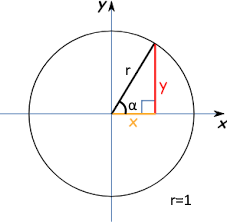
\includegraphics{resources/UnitCircle.png}

\subsection{正三角函数}{
  $\sin{\alpha} = \frac{y}{r}$

  $\cos{\alpha} = \frac{x}{r}$

  $\tan{\alpha} = \frac{y}{x}$
}
\subsection{反三角函数}{
  $\cot{\alpha} = \frac{1}{\tan{\alpha}}$

  $\sec{\alpha} = \frac{1}{\cos{\alpha}}$

  $\csc{\alpha} = \frac{1}{\sin{\alpha}}$
}

\subsection{和差化积}{
  $\sin{\alpha}+\sin{\beta} = 2\sin{\frac{\alpha + \beta}{2}}\cos{\frac{\alpha - \beta}{2}}$

  $\cos{\alpha}+\cos{\beta} = 2\cos{\frac{\alpha + \beta}{2}\cos{\frac{\alpha-\beta}{2}}}$

  $\cos{\alpha}-\cos{\beta} = -2\sin{\frac{\alpha + \beta}{2}}\cos{\frac{\alpha - \beta}{2}}$

  $\sin{\alpha}-\sin{\beta} = 2\sin{\frac{\alpha + \beta}{2}}\cos{\frac{\alpha - \beta}{2}}$
}

\subsection{积化和差}{
  $\cos{\alpha + \beta} = \cos{\alpha}\cos{\beta} - \sin{\alpha}\sin{\beta}$

  $\cos{\alpha - \beta} = \cos{\alpha}\cos{\beta} + \sin{\alpha}\sin{\beta}$

  $\sin{\alpha \pm \beta} = \sin{\alpha}\cos{\beta} \pm \cos{\alpha}\sin{\beta}$

  $\sin{\alpha}\cos{\beta} = \frac{1}{2}[\sin{(\alpha + \beta)} + \sin{(\alpha - \beta)}]$

  $\cos{\alpha}\cos{\beta} = \frac{1}{2}[\cos{(\alpha + \beta)} + \cos{(\alpha - \beta)}]$

  $\sin{\alpha}\sin{\beta} = -\frac{1}{2}[\cos{(\alpha + \beta)} - \cos{(\alpha - \beta)}]$
}

\subsection{诱导公式}{
  \indent 奇变偶不变,符号看象限。
  \subsubsection{第一组诱导公式}{
    $\sin{(2k\pi + \alpha)} = \sin{\alpha}$

    $\cos{(2k\pi + \alpha)} = \cos{\alpha}$

    $\tan(2k\pi + \alpha) = \tan\alpha$

    $\cot(2k\pi + \alpha) = \cot\alpha$
  }

  \subsubsection{第二组诱导公式}{
    $\sin(-\alpha) = -\sin\alpha$

    $\cos(-\alpha) = \cos\alpha$

    $\tan(-\alpha) = -\tan\alpha$

    $\cot(-\alpha) = -\cot\alpha$
  }

  \subsubsection{第三组诱导公式}{
    $\sin(\pi + \alpha) = -\sin\alpha$

    $\cos(\pi + \alpha) = -\cos\alpha$

    $\tan(\pi + \alpha) = \tan\alpha$

    $\cot(\pi + \alpha) = \cot\alpha$
  }

  \subsubsection{第四组诱导公式}{
    $\sin(\pi - \alpha) = \sin\alpha$

    $\cos(\pi - \alpha) = -\cos\alpha$

    $\tan(\pi - \alpha) = -\tan\alpha$

    $\cot(\pi - \alpha) = -\cot\alpha$
  }

  \subsubsection{第五组诱导公式}{
    $\sin(\frac{\pi}{2} - \alpha) = \cos\alpha$

    $\cos(\frac{\pi}{2} - \alpha) = \sin\alpha$

    $\tan(\frac{\pi}{2} - \alpha) = \cot\alpha$

    $\cot(\frac{\pi}{2} - \alpha) = \tan\alpha$
  }

  \subsubsection{第六组诱导公式}{
    $\sin(\frac{\pi}{2} + \alpha) = \cos\alpha$

    $\cos(\frac{\pi}{2} + \alpha) = -\sin\alpha$

    $\tan(\frac{\pi}{2} + \alpha) = -\cot\alpha$

    $\cot(\frac{\pi}{2} + \alpha) = -\tan\alpha$
  }

  \subsubsection{杂项}{
    $a\sin\alpha + b\cos\alpha = \sqrt{a^2 + b^2}\sin(\alpha+\beta)$
  }

}

\subsection{倍角公式}{
  \subsubsection{半倍角公式}{
    $\sin\frac{\alpha}{2} = \pm\sqrt{\frac{1 - \cos\alpha}{2}}$

    $\cos\frac{\alpha}{2} = \pm\sqrt{\frac{1 + \cos\alpha}{2}}$
  }
}

\subsection{三角恒等式}{
$\csc^2{x} - cot^2{x} = 1$

$\sec^2x - tan^2x = 1$ %去你🐎的大括号

$\sin^2x + \cos^2x = 1$

$\tan{x} = \frac{\sin{x}}{\cos{x}}$

}
\section{极限}{

  \subsection{定理}{
    \begin{enumerate}
      \item 函数在一点极限存在的条件是左右极限存在且相等
    \end{enumerate}
  }

  \subsection{重要极限}{
    {\myLimToZero$\frac{\sin{x}}{x}=1$} $\to$ {\limNormal{x \to 0}$\sin{x} \to x$}

      {\myLimToInf$(1+\frac{1}{x})^x = e$}
  }

 }

\end{document}